\documentclass[a4paper]{article}
\usepackage{geometry}
\geometry{
a4paper,
left=3cm, top=3cm,
bottom=2cm, right=2cm}
\usepackage[portuguese]{babel}
\usepackage[utf8]{inputenc}
\usepackage{amsmath}
\usepackage{graphicx}
\usepackage{tabularx}
\usepackage{fancyhdr}
\usepackage{times}
\usepackage[colorinlistoftodos]{todonotes}
\frenchspacing
\usepackage{array,booktabs}

\usepackage[nottoc]{tocbibind}
\usepackage[colorlinks=true,linkcolor=black]{hyperref}

\makeatletter
\title{Modelagem Conceitual de Dados} \let\Title\@title
\author{Alberto Oliveira da Silva\\ \texttt{orkan.aos@gmail.com} \\ \vspace{2.5mm}
Danilo Machado de Souza \\ \texttt{dan.machado.1989@gmail.com} \\ \vspace{2.5mm}
Guilherme Augusto Rodrigues Melo \\ \texttt{guilhermearmelo@gmail.com} \\ \vspace{2.5mm}
Luís Filipe Lima Alves Vieira \\ \texttt{luisflavieira@gmail.com}} \let\Author\@author
\date{\today} \let\Date\@date
\makeatother

\addto\captionsportuguese{\renewcommand*\contentsname{Sumário}}

\begin{document}
\begin{large}
\begin{titlepage}
  \begin{center}
    \textsc{
    \LARGE
    Universidade Federal de Ouro Preto\\
    \Large
    Instituto de Ciências Exatas e Biológicas \\
    Departamento de Computação \\
    BCC321 - Banco de Dados I \\
    Prof. Dr. Guilherme Tavares de Assis\\}
    \vspace*{5cm}
    \LARGE{\Title} \\
    \vspace*{4cm}
    \Large{\Author} \\
    \vspace{\fill}
    \textbf{\Date}
  \end{center}
\end{titlepage}

\tableofcontents
\clearpage
%\listoffigures
%\listoftables
%\clearpage

\section{Introdução}
\quad Este trabalho consiste na elaboração dos requisitos de dados de um sistema de banco de dados e do consequente esquema conceitual Entidade Relacionamento Estendido (ERE) de um provedor de infraestrutura. Sendo assim, consideramos o mini-mundo como o próprio provedor e modelamos suas possíveis entidades e relacionamentos com seus respectivos atributos.

%O trabalho consiste na elaboração dos requisitos de dados de um sistema de banco de dados e do
%consequente esquema conceitual Entidade Relacionamento Estendido (ERE). A documentação a ser
%entregue deve conter os seguintes itens:
%1) Descrição textual detalhada dos requisitos de dados do sistema.
%2) Esquema ERE completo dos dados do sistema, na notação adotada pelo livro texto. O esquema
%ERE deve conter, no mínimo, 10 entidades, uma hierarquia de especialização ou de
%generalização, uma união ou agregação.
%3) Dicionário de dados contendo uma descrição textual de cada entidade, relacionamento e
%atributo. Para cada entidade, devem ser especificadas a semântica da mesma e a lista de
%atributos que a caracterizam. Para cada atributo, devem ser especificados a semântica do
%mesmo, as categorias em que se enquadra e o domínio correspondente. Para cada
%relacionamento, devem ser especificadas as entidades envolvidas e as restrições estabelecidas
%de cardinalidade e parteção. 

\section{Descrição textual}
\quad Um provedor de infraestrutura trabalha fornecendo acesso a servidores que estão localizados em datacenters ao redor do mundo. Estes datacenters são classificados segundo o nível de qualidade de serviço que conseguem prover (Tier) e estão sitiados em um endereço cujas informações relevantes são apenas as de país, estado e cidade para efeitos de velocidade de transmissão pela internet. Os servidores possuem diversos componentes sendo que precisam ter no mínimo um de cada componente; estes componentes são CPU de determinado modelo com sua velocidade de clock, tamanho da cache, quantidade de núcleos e tipo(thread, core) definidos; RAM de determinado modelo com sua velocidade de acesso, tamanho da memória e tipo da memória (DDR1, DDR2, etc); GPU de determinado modelo com seu clock de núcleo, clock da memória, tamanho da memória e tipo (GDDR5, etc); e Disco de determinado modelo com sua capacidade de armazenamento, velocidade de escrita, velocidade de leitura e tipo (HDD, SSD).
\par Para ter acesso a um servidor é preciso pagar por uma taxa mensal ou por uso de cada hora sendo estas taxas especificadas no momento que um cliente aluga um servidor. O cliente pode tanto ser uma pessoa física com o cadastro de seu CPF ou uma pessoa jurídica com o cadastro de seu CNPJ; fora isso, esses dois tipos de cliente apresentam detalhes em comum que também devem ser cadastrados como: um registro único que o identifica, uma forma de contato composta de email e um ou mais números de telefone, e endereço composto de país, estado, cidade, código postal, rua e número da residência além de uma ou mais formas de pagamento. Este cliente é então capaz de abrir chamados(tickets) de suporte, reclamação, ou outra categoria de atendimento; este ticket deve possuir um código que o identifique, a descrição feita pelo cliente do que deve ser feito ou do problema ocorrido, deve ser registrado a data de abertura do ticket bem como sua data de resolução/fechamento; é permitido que tanto o cliente quanto o funcionário responsável pelo atendimento façam comentários no ticket.
\par Um funcionário da empresa (provedora de infraestrutura) é capaz de resolver um ticket e marcá-lo como concluído. O funcionário tem que estar cadastrado e ter informações de seu SSN (Social Security Number) que similar ao CPF é único para cada pessoa, de sua data de entrada na empresa bem como seu cargo. O funcionário deve também ter registrado seu nome, seu salário e uma forma de contato composta de email e um ou mais telefones.
\section{Esquema ERE}
\end{large}
\clearpage

\newgeometry{left=0cm,top=0cm,bottom=0cm,right=0cm}
\addtocounter{page}{-1}
\begin{center}
\begin{figure}[!ht]
\noindent\makebox[\textwidth]{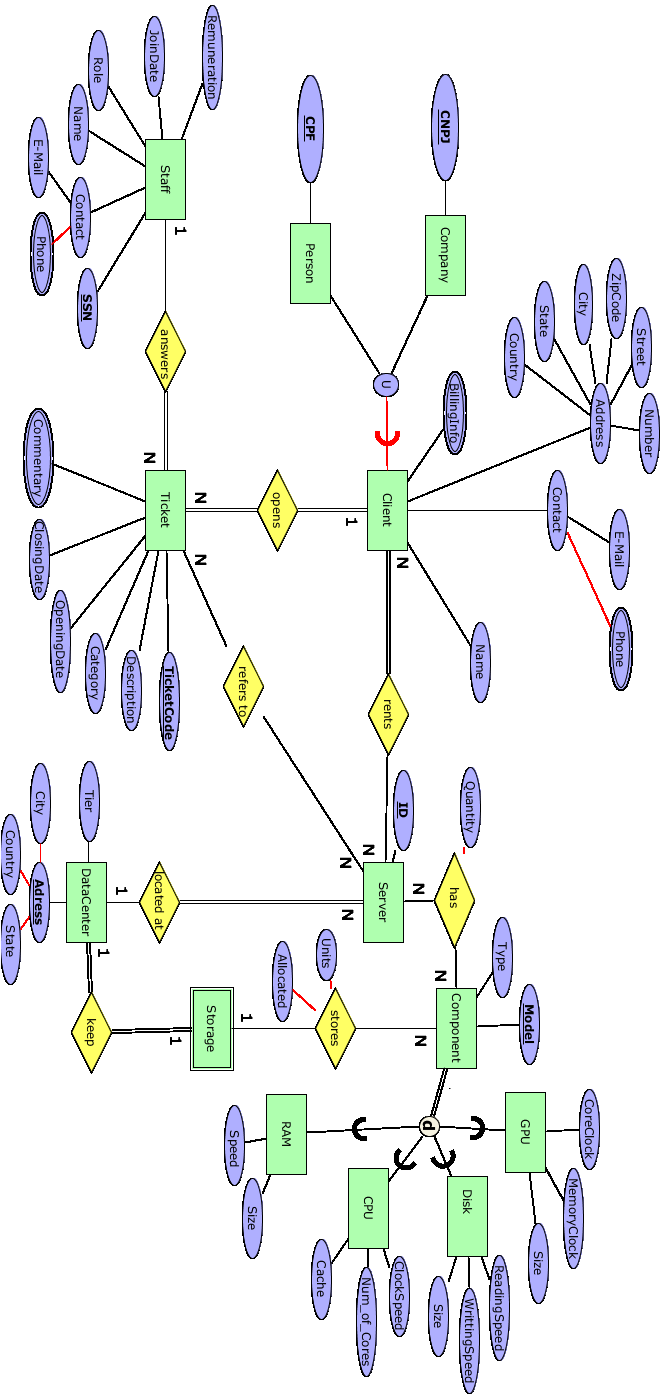
\includegraphics[width=\paperwidth, height=0.99\paperheight]{diagrama.png}}
\end{figure}
\end{center}
\pagebreak
\restoregeometry

\newgeometry{top=3cm,bottom=2cm, right=2cm, left=3cm}
\begin{large}
\section{Dicionário de dados}
\quad Por padrão, admite-se que os atributos sejam simples, mono-valorados e armazenados. Assim, faz-se necessário apenas ressaltar o tipo quando divergir deste padrão. (Obs: Para efeitos de completude da tabela, os atributos que seguem o padrão apresentam "simples" na coluna de tipo). \\
\end{large}
\renewcommand{\arraystretch}{1.5}
\begin{center}
\begin{table}[ht]
\begin{tabularx}{\textwidth}{|c|c|c|X|} \hline
\multicolumn{4}{|c|}{\shortstack{\textbf{Client: entidade que representa o cliente do provedor com seus dados de cadastro	}}} \\ \hline
\textit{Atributo} & \textit{Tipo} & \textit{Descrição} & \textit{Observação} \\ \hline
BillingInfo & multi-valorado & método(s) de pagamento do cliente & - \\ \hline
Address & composto & endereço do cliente & - \\ \hline
Country & simples & país do cliente & parte do atributo composto \textit{Address} \\ \hline
State & simples & estado do cliente & parte do atributo composto \textit{Address} \\ \hline
City & simples & cidade do cliente & parte do atributo composto \textit{Address} \\ \hline
ZipCode & simples & CEP do cliente & parte do atributo composto \textit{Address} \\ \hline
Street & simples & rua do cliente & parte do atributo composto \textit{Address} \\ \hline
Number & simples & número da residência do cliente & parte do atributo composto \textit{Address} \\ \hline
Contact & composto & dados de contato do cliente & - \\ \hline
Email & simples & email do cliente & parte do atributo composto \textit{Contact} \\ \hline
Phone & multi-valorado & telefone(s) do cliente & parte do atributo composto \textit{Contact} \\ \hline
Name & simples & nome do cliente & - \\ \hline
\multicolumn{4}{|c|}{\shortstack{\textbf{ Relacionamentos }}} \\ \hline
\multicolumn{4}{|c|}{\shortstack{Client é uma união de Company e Person portanto sua chave primária é herdada deles}} \\ \hline
\end{tabularx}
\end{table}

\begin{table}[ht]
\begin{tabularx}{\textwidth}{|c|c|c|X|} \hline
\multicolumn{4}{|c|}{\shortstack{\textbf{Company: entidade que representa um cliente que é uma pessoa jurídica (empresa) }}} \\ \hline
\textit{Atributo} & \textit{Tipo} & \textit{Descrição} & \textit{Observação} \\ \hline
CNPJ & simples & CNPJ da pessoa jurídica (empresa)  & - \\ \hline
\end{tabularx}
\end{table}

\begin{table}[ht]
\begin{tabularx}{\textwidth}{|c|c|c|X|} \hline
\multicolumn{4}{|c|}{\shortstack{\textbf{Person: entidade que representa um cliente que é uma pessoa física (pessoa) }}} \\ \hline
\textit{Atributo} & \textit{Tipo} & \textit{Descrição} & \textit{Observação} \\ \hline
CPF & simples & CPF da pessoa física (pessoa) & - \\ \hline
\end{tabularx}
\end{table}

\newgeometry{top=5cm,bottom=0cm, right=2cm, left=3cm}

\begin{table}[ht]
\begin{tabularx}{\textwidth}{|c|c|c|X|} \hline
\multicolumn{4}{|c|}{\shortstack{\textbf{Ticket: entidade que representa um ticket que o cliente abre para receber suporte }}} \\ \hline
\textit{Atributo} & \textit{Tipo} & \textit{Descrição} & \textit{Observação} \\ \hline
TicketCode & chave & código de identificação do ticket & - \\ \hline
Description & simples & descrição do ticket & - \\ \hline
Category & simples & categoria do ticket (suporte, compras, reclamação) & - \\ \hline
Commentary & multi-valorado & comentário(s) trocado(s) entre cliente e funcionário & - \\ \hline
OpeningDate & simples & data de abertura do ticket & - \\ \hline
ClosingDate & simples & data de conclusão do ticket & - \\ \hline
\multicolumn{4}{|c|}{\shortstack{\textbf{ Relacionamentos }}} \\ \hline
OpenedBy & chave estrangeira & identificação do cliente que abriu o ticket & relação \textit{opens} \\ \hline
SolvedBy & chave estrangeira & identificação do funcionário que resolveu o ticket & relação \textit{solves} \\ \hline
RefersTo & chave(s) estrangeira(s) & identificação do(s) servidor(es) referentes ao ticket & relação \textit{refers} \\ \hline
\end{tabularx}
\end{table}

\begin{table}[ht]
\begin{tabularx}{\textwidth}{|c|c|c|X|} \hline
\multicolumn{4}{|c|}{\shortstack{\textbf{Staff: entidade que representa um funcionário do provedor }}} \\ \hline
\textit{Atributo} & \textit{Tipo} & \textit{Descrição} & \textit{Observação} \\ \hline
Contact & composto & dados de contato do funcionário & - \\ \hline
Email & simples & email do funcionário & parte do atributo composto \textit{Contact} \\ \hline
Phone & multi-valorado & telefone(s) do funcionário & parte do atributo composto \textit{Contact} \\ \hline
Name & simples & nome do funcionário & - \\ \hline
Remuneration & simples & salário do funcionário & - \\ \hline
JoinDate & simples & data de contrato & - \\ \hline
Role & simples & cargo do funcionário & - \\ \hline
SSN & chave & Social Security Number & - \\ \hline
\end{tabularx}
\end{table}

\begin{table}[ht]
\begin{tabularx}{\textwidth}{|c|c|c|X|} \hline
\multicolumn{4}{|c|}{\shortstack{\textbf{Server: entidade que representa um servidor do provedor }}} \\ \hline
\textit{Atributo} & \textit{Tipo} & \textit{Descrição} & \textit{Observação} \\ \hline
IP & simples & endereço IP atribuído ao servidor & - \\ \hline
MACAddress & chave & identificador único do servidor & - \\ \hline
OperationalSystem & simples & sistema operacional instalado no servidor & - \\ \hline
MonthlyCost & simples & custo mensal do servidor & - \\ \hline
HourlyCost & simples & custo por hora do servidor & - \\ \hline
\multicolumn{4}{|c|}{\shortstack{\textbf{ Relacionamentos }}} \\ \hline
Components & chaves estrangeiras & modelos dos componentes do servidor & relação \textit{has} \\ \hline
LocatedAt & chave estrangeira & identificação do datacenter onde está servidor & relação \textit{locatedat} \\ \hline
RentedBy & chave estrangeira & identificação do cliente que alugou o servidor & relação \textit{rents} \\ \hline
\end{tabularx}
\end{table}

\begin{table}[ht]
\begin{tabularx}{\textwidth}{|c|c|c|X|} \hline
\multicolumn{4}{|c|}{\shortstack{\textbf{Datacenter: entidade que representa um datacenter do provedor }}} \\ \hline
\textit{Atributo} & \textit{Tipo} & \textit{Descrição} & \textit{Observação} \\ \hline
Address & chave composta & endereço do datacenter & - \\ \hline
Country & simples & país do datacenter & parte da chave composta \textit{Address} \\ \hline
State & simples & estado do datacenter & parte da chave composta \textit{Address} \\ \hline
City & simples & cidade do datacenter & parte da chave composta \textit{Address} \\ \hline
\multicolumn{4}{|c|}{\shortstack{\textbf{ Relacionamentos }}} \\ \hline
Keep & chave estrangeira & identificação do storage do datacenter & - \\ \hline
\end{tabularx}
\end{table}

\begin{table}[ht]
\begin{tabularx}{\textwidth}{|c|c|c|X|} \hline
\multicolumn{4}{|c|}{\shortstack{\textbf{Storage: entidade fraca que representa um warehouse no datacenter }}} \\ \hline
\textit{Atributo} & \textit{Tipo} & \textit{Descrição} & \textit{Observação} \\ \hline
Allocated & simples & disponibilidade de componente & parte da relação \textit{stores} \\ \hline
Units & simples & unidades de componentes & parte da relação \textit{stores} \\ \hline
\multicolumn{4}{|c|}{\shortstack{\textbf{ Relacionamentos }}} \\ \hline
stores & chave(s) estrangeira(s) & identificação dos componentes guardados & - \\ \hline
\end{tabularx}
\end{table}

\begin{table}[ht]
\begin{tabularx}{\textwidth}{|c|c|c|X|} \hline
\multicolumn{4}{|c|}{\shortstack{\textbf{CPU: entidade que representa um modelo de CPU (processador) }}} \\ \hline
\textit{Atributo} & \textit{Tipo} & \textit{Descrição} & \textit{Observação} \\ \hline
Model & chave & modelo da CPU & - \\ \hline
Type & simples & tipo de CPU (thread/core) & - \\ \hline
ClockSpeed & simples & velocidade de Clock da CPU & - \\ \hline
Cores & simples & quantidade de núcleos da CPU & - \\ \hline
Cache & simples & tamanho da cache da CPU & - \\ \hline
\end{tabularx}
\end{table}

\begin{table}[ht]
\begin{tabularx}{\textwidth}{|c|c|c|X|} \hline
\multicolumn{4}{|c|}{\shortstack{\textbf{RAM: entidade que representa um modelo de RAM (memória de acesso aleatório)}}} \\ \hline
\textit{Atributo} & \textit{Tipo} & \textit{Descrição} & \textit{Observação} \\ \hline
Model & chave & modelo da RAM & - \\ \hline
Type & simples & tipo de RAM (DDR/DDR2/../DDR5) & - \\ \hline
Size & simples & tamanho em MB da RAM & - \\ \hline
Speed & simples & velocidade de acesso da RAM & - \\ \hline
\end{tabularx}
\end{table}

\begin{table}[ht]
\begin{tabularx}{\textwidth}{|c|c|c|X|} \hline
\multicolumn{4}{|c|}{\shortstack{\textbf{GPU: entidade que representa um modelo de GPU (placa gráfica) }}} \\ \hline
\textit{Atributo} & \textit{Tipo} & \textit{Descrição} & \textit{Observação} \\ \hline
Model & chave & modelo da GPU & - \\ \hline
Type & simples & tipo de GPU (GDDR5) & - \\ \hline
Size & simples & tamanho em MB da GPU & - \\ \hline
CoreClock & simples & frequência de clock dos núcleos da GPU & - \\ \hline
MemoryClock & simples & frequência de clock da memória da GPU & - \\ \hline
\end{tabularx}
\end{table}

\begin{table}[ht]
\begin{tabularx}{\textwidth}{|c|c|c|X|} \hline
\multicolumn{4}{|c|}{\shortstack{\textbf{Disk: entidade que representa um modelo de disco }}} \\ \hline
\textit{Atributo} & \textit{Tipo} & \textit{Descrição} & \textit{Observação} \\ \hline
Model & chave & modelo do disco & - \\ \hline
Type & simples & tipo do disco (HDD/SSD) & - \\ \hline
Size & simples & tamanho em GB de armazenamento do disco & - \\ \hline
WritingSpeed & simples & velocidade de escrita do disco & - \\ \hline
ReadingSpeed & simples & velocidade de leitura do disco & - \\ \hline
\end{tabularx}
\end{table}

\end{center}

\end{document}